\documentclass{article}

\title{Machine Learning in the Detection of Intracranial Hemorrhages from Head CT Scans}
\author{Peter Tran}
\date{}

\usepackage{amsmath}
\usepackage{graphicx}
\graphicspath{ {./figures/} }
\setlength{\parskip}{1em}

\begin{document}

\maketitle

\begin{abstract}
    Head CT scans are the primary imaging tool used to identify important features in the event of stroke screening. Rapid and accurate detection of hemorrhages is necessary to determine the course of treatment and stabilize patients. In this experiment, we develop a CNN model for detecting any kind of intracranial hemorrhage from a CT scan using a dataset of \textasciitilde650,000 images. Our final model was able to get a mean $F_2$ score of 0.492 +/- 0.232 under 5-fold cross-validation, and on a 20\% holdout test set, we got an $F_2$ score of 0.648. This demonstrates the efficacy of deep learning and CNNs in head CT analysis and can help pave the way towards automated and accurate detection of emergent strokes.
\end{abstract}

\section{Introduction}
    Computed tomography (CT) scans are the first line of defense in emergency rooms for dealing with patients presenting with stroke symptoms and history. Traditionally, after a CT scan is performed, it is read by a team of radiologists who identify critical features to determine the best clinical plan; in particular, the detection of an existing intracranial hemorrhage must occur to rule out the use of thrombolytics to treat ischemic strokes, which are the vast majority (87\%) of strokes \cite{Dariush}. Administering thrombolytics in the case of a hemorrhagic stroke is fatal, and an intracranial hemorrhage does damage quickly and requires swift intervention. However, this process must be fast because the faster a thrombolytic can be administered in the case of ischemic stroke, the more brain tissue can be saved \cite{Ebinger}\cite{Fonarow}\cite{Strbian}. Therefore, there is a significant need to speed up this process as much as possible. This paves way for the use of machine learning to perform rapid, automated detection of critical features in head CT scans.
    
    We investigate the use of convolutional neural networks (CNNs) in this domain, as they are particularly effective in medical image analysis \cite{Anwar}. For this experiment, we focus on the detection of hemorrhages as they tend to cause much more drastic changes in CT images [Fig. \ref{fig:ischemic_vs_hemorrhagic}] and the window for treatment is much thinner than in cases of ischemic stroke. To develop such a model, we use a dataset of head CTs labeled with whether a hemorrhage exists and what type it is. The data is from the Radiological Society of North America and can be found on Kaggle \cite{Kaggle}.
    
\begin{figure}[]
    \centering
    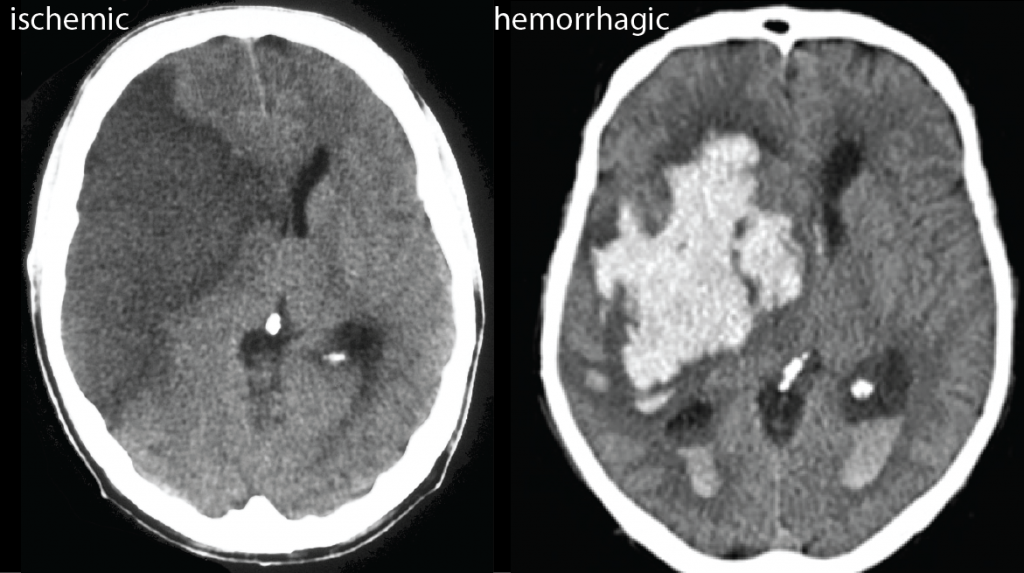
\includegraphics[width=8cm]{ischemic_vs_hemorrhagic}
    \caption{Ischemic vs hemorrhagic CT scans. On visual inspection, to us it appears that hemorrhagic strokes cause much larger changes in the CT image from a healthy brain compared to an ischemic stroke. Image source: \cite{Stroke_Comparison}}
    \label{fig:ischemic_vs_hemorrhagic}
\end{figure}

\section{Methods}
    Before we can begin developing our model, we had to download the data and do some preprocessing. The dataset contained 753,803 images in DICOM format. Each image had an identifier with five different types of hemorrhages that may exist in an image: intraparenchymal, intraventricular, subarachnoid, subdural, and epidural. Instead of tackling a multi-label classification problem, we decided to start simple and just try to predict whether an image has any of these hemorrhages or not. The dataset is slightly imbalanced [Fig. \ref{fig:any_hemo_count}] with 644,870 images in the negative case and 107,933 in the positive case. The imbalance is small enough that weighting the loss function should be enough. During image preprocessing, several images were unable to be read and a few were a different size from the majority size (512 by 512 pixels), those images were discarded leaving a final dataset size of 752,533 images. After preprocessing, 20\% of the images were set aside to use as the holdout test set for the final evaluation of our model. That left us with 602,026 images to train models with.
    
\begin{figure}[]
    \centering
    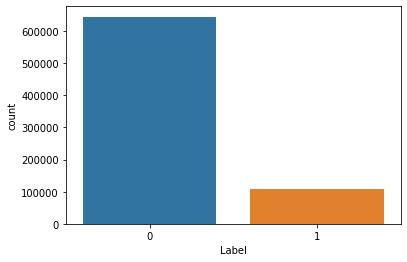
\includegraphics[width=8cm]{any_hemo_count}
    \caption{Any hemorrhage counts. Count of hemorrhage existence in each image. A label of 0 is no hemorrhage detected, and 1 is a hemorrhage detected.}
    \label{fig:any_hemo_count}
\end{figure}

    To evaluate model performance, we had to select a metric. We decided to use the $F_2$ score [Eq. 1]. The $F_2$ score is similar to the $F_1$ score, where it is the harmonic mean between specificity and sensitivity, but sensitivity is considered twice as important. This was decided because the model is slightly imbalanced, so accuracy would not be a good metric to use, and in a clinical environment, it is much more important to detect as many true positives as possible, even at the expense of some false positives.
    
\begin{equation}
    F_2 = 5 \cdot \frac{\text{specificity} \cdot \text{sensitivity}}{4 \cdot \text{specificity} + \text{sensitivity}}
    \label{eq:1}
\end{equation}
    
    Since the training dataset was so large (takes up almost 500Gb of RAM to hold in memory), a generator had to be created to load data on-demand as models required in batches. Also, a framework was developed to allow for rapid model evaluation so that each model's performance can be quickly estimated with a random stratified sampling of the training dataset. 10 models were developed and quickly evaluated, where each one had it's $F_2$ score calculated as well as accuracy, sensitivity, and specificity [Tab. \ref{tab:quick_evaluation}]. Loss curves were also plotted, and used to determine how to tweak a model or what architecture to try next. Models were trained with varying sizes of samples, depending on the training time and complexity of the model. The average size was about 30,000 images. Almost all models trained use the CNN architecture. The basic algorithm behind CNNs is to set a window size and translate that window over the image (convolution) with user-defined step size, extracting those features (called filters), then you pool all these filters together into a smaller space defined by the user by selecting the most important features, usually done by selecting the maximum or average values. In every case, we are pooling by maximum values.

\begin{table}[]
    \centering
    \makebox[\textwidth]{%
    \begin{tabular}{|l|l|l|l|l|}
        \hline
        Candidate & F2                  & Accuracy            & Sensitivity         & Specificity         \\ \hline
        m1        & 0.5360824742268042  & 0.478               & 0.9059233449477352  & 0.20360219263899765 \\ \hline
        m2        & 0.27452415812591513 & 0.8225              & 0.2613240418118467  & 0.3440366972477064  \\ \hline
        m3        & 0.0                 & 0.8565              & 0.0                 & 0.0                 \\ \hline
        m4        & 0.46023091725465043 & 0.1585              & 1.0                 & 0.14568527918781726 \\ \hline
        m5        & 0.4577157802964254  & 0.8053333333333333  & 0.4883720930232558  & 0.36585365853658536 \\ \hline
        m6        & 0.4555084745762712  & 0.14333333333333334 & 1.0                 & 0.14333333333333334 \\ \hline
        m7        & 0.5818181818181818  & 0.797               & 0.6697674418604651  & 0.38145695364238413 \\ \hline
        m8        & 0.4203792551976239  & 0.8231666666666667  & 0.42790697674418604 & 0.3927427961579509  \\ \hline
        m9        & 0.5938308090136682  & 0.7418333333333333  & 0.7479643272586274  & 0.3255146810664867  \\ \hline
        m10       & 0.6188475390156063  & 0.7333888888888889  & 0.7995347033734005  & 0.325031525851198   \\ \hline
    \end{tabular}}
    \caption{Quick evaluation scores.}
    \label{tab:quick_evaluation}
\end{table}

    After developing and quickly evaluating several models, 5-fold cross-validation was performed on 100,000 samples to ensure the statistical performance of the best model. m10 was selected for the highest performance, and based on the loss curve it should not overfit too quickly with enough samples. Once satisfied with cross-validation, the model was retrained on 300,000 samples and early stopping was used to get the best weights before the model overfits on training data. The model is then evaluated by plotting its specificity-sensitivity curve, and the best threshold for $F_2$ score is computed based on the training data. The model is then evaluated on the holdout test set, using the calculated threshold. The full experimental pipeline can be seen in [Fig. \ref{fig:pipeline}]
    
\begin{figure}[]
    \centering
    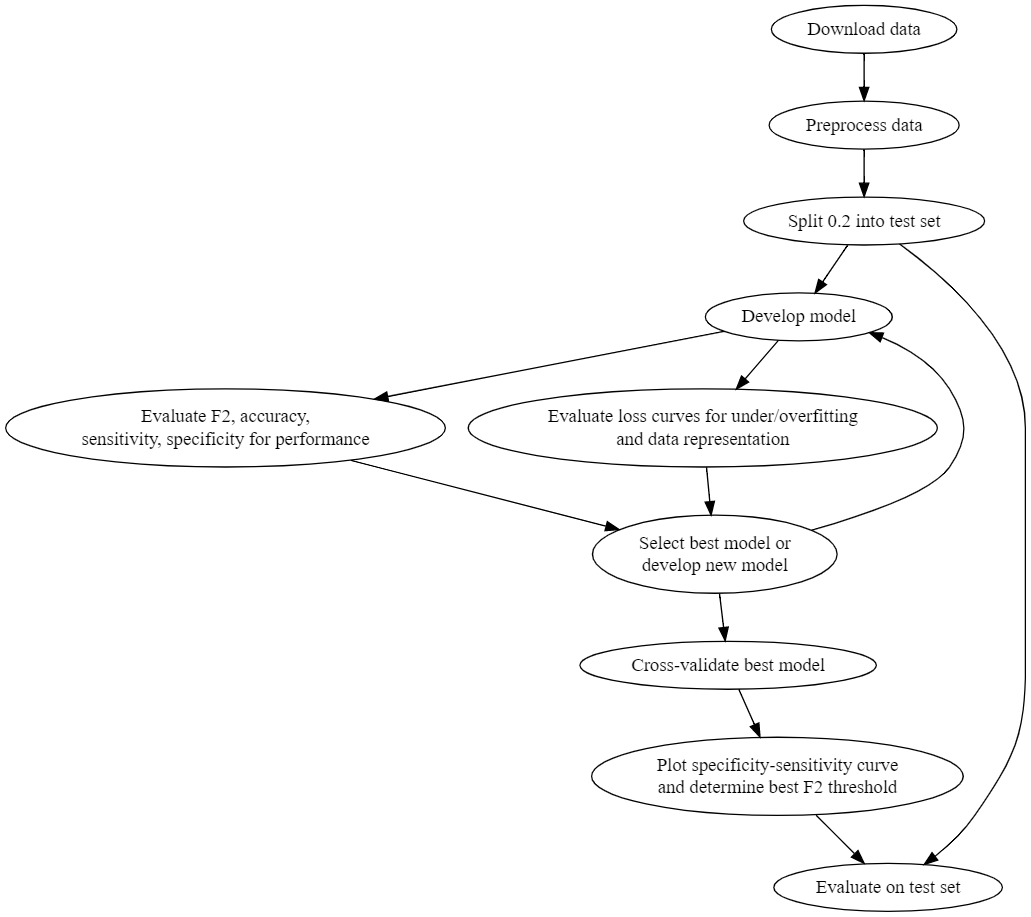
\includegraphics[width=14cm]{pipeline}
    \caption{Experimental pipeline.}
    \label{fig:pipeline}
\end{figure}
    
\clearpage
\section{Results}

    m10 performs well under cross-validation with a mean $F_2$ of 0.492 +/- 0.232 and mean accuracy of 0.795 +/- 0.035. The variance of the $F_2$ score is much higher than we would prefer, but since the final model will be trained on larger sample size, the variance should shrink; also we will be able to adjust the specificity-sensitivity threshold to maximize the $F_2$ score. The model architecture can be seen in [Fig. \ref{fig:architecture}]
    
\begin{figure}[]
    \centering
    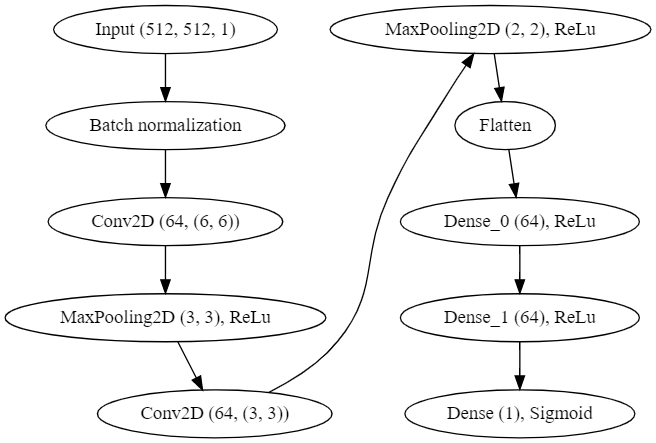
\includegraphics[width=8cm]{architecture}
    \caption{Architecture of m10.}
    \label{fig:architecture}
\end{figure}
    
\begin{figure}[]
    \centering
    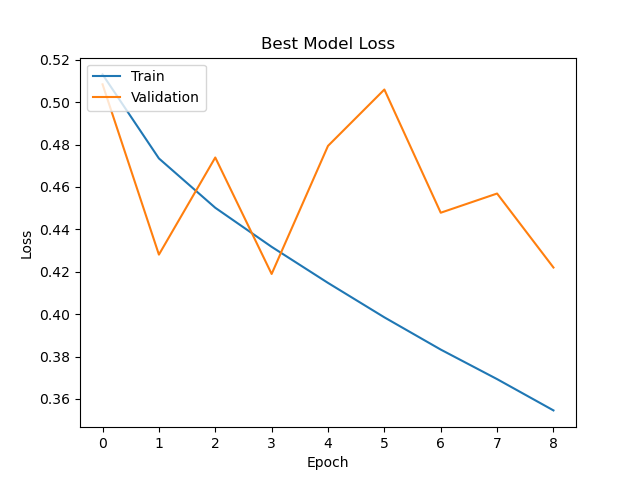
\includegraphics[width=8cm]{best_model_loss}
    \caption{Loss curve of m10.}
    \label{fig:best_model_loss}
\end{figure}
    
    The loss curve for the final model can be seen in [Fig. \ref{fig:best_model_loss}]. The training loss smoothly decreases and appears to be able to continue to decrease with additional training, but the validation loss begins increasing after the fourth epoch. It appears the model begins to overfit on the training data then. It's also extremely variable and does not appear the validation data sample is large enough. Early stopping was used, and the weights where the validation loss was the lowest were selected. We move on to plot the specificity-sensitivity curve to help identify where we might want to set our threshold [Fig. \ref{fig:best_model_precision_recall}]. Upon visual examination, it looks like not too far from 0.5 is a good threshold. We calculated the $F_2$ scores for each threshold and determined that 0.420 maximizes it. We use that threshold in evaluating the model with the holdout test set and get an $F_2$ score of 0.648 and an accuracy of 0.77, the confusion matrix is in [Fig. \ref{fig:best_model_confusion_matrix}].
    
\begin{figure}[]
    \centering
    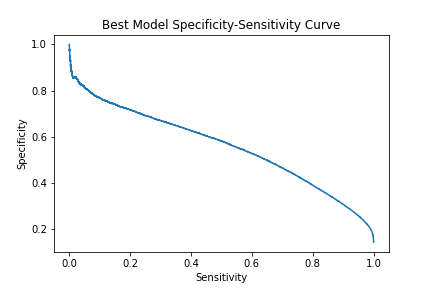
\includegraphics[width=8cm]{best_model_precision_recall}
    \caption{Specificity-sensitivity curve of m10.}
    \label{fig:best_model_precision_recall}
\end{figure}

\begin{figure}[]
    \centering
    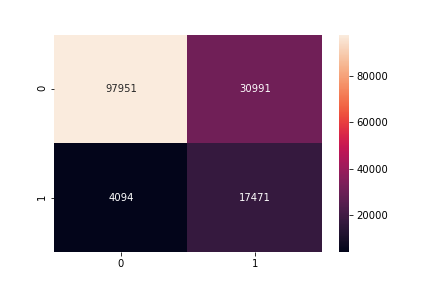
\includegraphics[width=8cm]{best_model_confusion_matrix}
    \caption{Confusion matrix of m10 on holdout test dataset. The x-axis is predicted values, and the y-axis is true values; 0 means no hemorrhage was found and 1 means there was one found.}
    \label{fig:best_model_confusion_matrix}
\end{figure}
    
\newpage
\section{Discussion}

    In the end, our model performs decently well. However, it overfits earlier than expected, even with a large sample size of 300,000 samples. In the future, we would like to use the full training set to train the model, as we believe that would prevent overfitting longer, and thus allow our model to generalize better. 300,000 was chosen for time purposes, as using the full \textasciitilde600,000 image dataset across 20 epochs would result in training the model for over 20 hours. When the experiment was begun, training was attempted on a CPU using a high-performance cluster, but it was far too slow. Moving the data onto a computer with a GPU easily increase training velocity by almost an order of magnitude larger. The loss curves (especially in the case of validation) were often very jittery. We believe this is due to the low sample size as well, as the final model's loss curve was much more smooth than the others. Regularization was also attempted with some models with dropout, but we saw very low performance as the network was unable to learn anything and presented a flat loss curve [Fig. \ref{fig:dropout}]. However, that was on a small sample size; if we were to train the full dataset with dropout, we may see overfitting holding off until much later and can squeeze several more epochs out of training. We also want to investigate using cross-validation for evaluation of all models on the full dataset; this would be slow, of course, but given enough time this would give us a much better impression of which models performed well and how. We did not attempt any under/oversampling, as the imbalance was not too great, but that would be a great experiment to see if those techniques would boost performance even further. We believe results can be improved greatly with more substantial preprocessing. Many images have skulls that are not centered or the same size in the frame, the coloring is not uniform, there is some noise in the data that can be filtered, and we could do some segmentation to extract only the brain and not the skull.

\begin{figure}[]
    \centering
    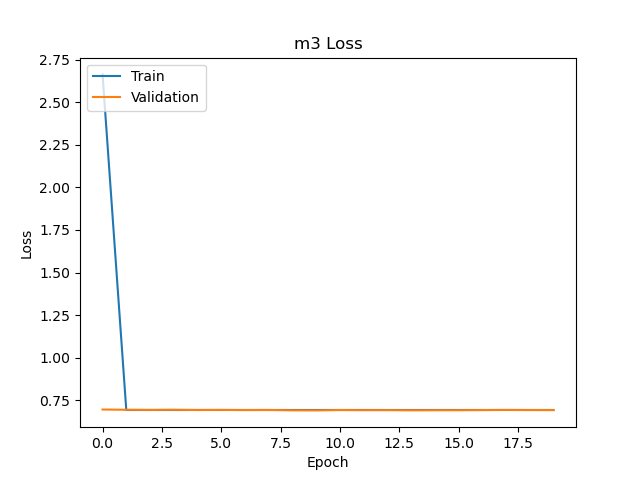
\includegraphics[width=8cm]{dropout}
    \caption{Loss curve of a model trained with dropout.}
    \label{fig:dropout}
\end{figure}

\clearpage
\bibliography{report}{}
\bibliographystyle{unsrt}

\end{document}
